\chapter{Comparison with exploding/vanishing gradients} \label{compare}

In this section, we explore whether the \textit{vanishing node} phenomenon arises from the problem of  exploding/vanishing gradients. Exploding/vanishing gradients in deep neural networks are a problem regarding the scale of forward-propagated signals and back-propagated gradients that exponentially explode/vanish as the networks grows deeper. We perform a theoretical analysis of exploding/vanishing gradients and show analytically the difference between them.
%it and the \textit{vanishing node} phenomena.


%We will first discuss the exploding/vanishing gradients problem via the theoretical model used in Section \ref{why}. We compare exploding and vanishing gradients problem with vanishing node phenomena analytically. Finally, we provide some numerical results to show the difference between exploding/vanishing gradients problem and vanishing node phenomena.

As in a previous study \cite{xavier}, we use the variances of hidden nodes to evaluate the scales of back-propagated gradients. Consider the model and the assumptions in Section \ref{why} and an additional assumption: the gradient of output layer $\frac{\partial Cost}{\partial \mathbf{x}_L}$ is a zero-mean i.i.d. random (row) vector.
That is,
\begin{equation}
    \begin{aligned}
    \mathbb{E}[\mathbf{x}_0{\mathbf{x}_0}^T] &= \sigma_x^2\cdot\mathbf{I} \\
    \mathbb{E}\Big[\Big(\frac{\partial Cost}{\partial \mathbf{x}_L}\Big)^T\frac{\partial Cost}{\partial \mathbf{x}_L}\Big] 
    &= \sigma_y^2\cdot\mathbf{I},
    \end{aligned}
\end{equation}
where $\sigma_x^2$ and $\sigma_y^2$ are defined as the variances of the input layer nodes and output layer gradients, respectively.
Consider %the forward and backward end-to-end propagation of variances, that is, 
the variances of the output nodes $Var[\mathbf{x}_L]$ and input layer gradients $Var\Big[\frac{\partial Cost}{\partial \mathbf{x}_0}\Big]$, respectively.
The exploding/vanishing gradients  occur only if the scales of forward and backward propagation exponentially increase or decrease as the depth increases.
This means that the magnitude of the gradients will be bounded if we can prevent the scales of forward and backward propagation from exploding or vanishing. 
%Therefore, we can keep forward and backward end-to-end propagation of variances from exploding or vanishing in order to avoid exploding and vanishing gradients problem.

According to the assumptions in Section \ref{why} and  \eqref{covariance_eqn},
we can approximate the shared scalar variance of all output nodes $Var[\mathbf{x}_L]\in\mathbb{R}$ as

\begin{equation}
    \begin{aligned}
    Var[\mathbf{x}_L] &=\mathbb{E}[(\mathbf{x}_L-\overline{\mathbf{x}_L})^T(\mathbf{x}_L-\overline{\mathbf{x}_L})]/N
    \approx \mathbb{E}[(\mathbf{Jx}_0)^T\mathbf{Jx}_0]/N\\
    &=\mathbb{E}[tr(\mathbf{J}^T\mathbf{J}\mathbf{x}_0\mathbf{x}_0^T)]/N
    =\sigma_x^2\cdot tr(\mathbf{J}^T\mathbf{J})/N,
    \label{xvar_to_trace}
    \end{aligned}
\end{equation}
and approximation the shared scalar variance of all input gradients $Var\Big[\frac{\partial Cost}{\partial \mathbf{x}_0}\Big]\in\mathbb{R}$ as

\begin{equation}
    \begin{aligned}
    Var\Big[\frac{\partial Cost}{\partial \mathbf{x}_0}\Big]
    &=\mathbb{E}\Big[\Big(\frac{\partial Cost}{\partial \mathbf{x}_0}-\overline{\frac{\partial Cost}{\partial \mathbf{x}_0}}\Big)
    \Big(\frac{\partial Cost}{\partial \mathbf{x}_0}-\overline{\frac{\partial Cost}{\partial \mathbf{x}_0}}\Big)^T\Big]\Big/N
    \\
    &= \mathbb{E}\Big[
    \Big(\frac{\partial Cost}{\partial \mathbf{x}_L}\mathbf{J}\Big)
    \Big(\frac{\partial Cost}{\partial \mathbf{x}_L}\mathbf{J}\Big)^T\Big]\Big/N
    \\
    &=\mathbb{E}\Big[tr\Big(\mathbf{J}\mathbf{J}^T\frac{\partial Cost}{\partial \mathbf{x}_L}^T\frac{\partial Cost}{\partial \mathbf{x}_L}\Big)\Big]/N
    \\
    &=\sigma_y^2\cdot tr(\mathbf{J}^T\mathbf{J})/N,
    \end{aligned}
    \label{yvar_to_trace}
\end{equation}
where the chain rule for back-propagation: $\frac{\partial Cost}{\partial \mathbf{x}_0}=\frac{\partial Cost}{\partial \mathbf{x}_L}\frac{\partial \mathbf{x}_L}{\partial \mathbf{x}_0}=\frac{\partial Cost}{\partial \mathbf{x}_L}\mathbf{J}$ is used, and the shared scalar variance of a vector is the average of the variances of all vector components.
Note that because the product of a row vector and a column vector is a scalar, the product is equal to its trace. Also, it is already known that
$tr(\mathbf{J}^T\mathbf{J})=N\cdot m_1=N\cdot(\sigma_w^2\mu_1)^L$. Thus, we have
\begin{equation}
    \begin{aligned}
    Var[\mathbf{x}_L]&\approx\sigma_x^2(\sigma_w^2\mu_1)^L\\
    Var\Big[\frac{\partial Cost}{\partial \mathbf{x}_0}\Big]&=\sigma_y^2(\sigma_w^2\mu_1)^L,
    \end{aligned}
\end{equation}
where $\sigma_w^2=N\cdot Var[W_{ij}]$, and $\mu_1$ is the first moment of the nonlinear activation function. It is obvious that the variances of both forward and backward propagation will neither explode nor vanish if and only if $(\sigma_w^2\mu_1)=1$.

For the weight gradient of the hidden layer $l$, the variance can be used to measure the scale distribution. Because $\frac{\partial Cost}{\partial \mathbf{W}_l}
=\mathbf{x}_{l-1}\cdot\frac{\partial Cost}{\partial \mathbf{h}_l}$ and both $\mathbf{x}_{l-1}$ and $\frac{\partial Cost}{\partial \mathbf{h}_l}$ are assumed to be zero-mean and independent of each other, the variance of the weight gradient can be evaluated as

\begin{equation}
    \begin{aligned}
    Var\Big[\frac{\partial Cost}{\partial \mathbf{W}_l}\Big]
    &=
    Var[\mathbf{x}_{l-1}]\cdot
    Var\Big[\frac{\partial Cost}{\partial \mathbf{h}_l}\Big]\\
    &
    \approx
    \sigma_x^2(\sigma_w^2\mu_1)^{l-1}\cdot
    \sigma_y^2(\sigma_w^2\mu_1)^{L-l}\\
    &=
    \sigma_x^2\sigma_y^2(\sigma_w^2\mu_1)^{L-1},
    \end{aligned}
    \label{weight_var}
\end{equation}
where we can evaluate $Var[\mathbf{x}_{l-1}]$ and $Var\Big[\frac{\partial Cost}{\partial \mathbf{h}_l}\Big]$ using the results of the forward/backward variance propagation and split the entire network into two sub-networks. One sub-network has the input layer $\mathbf{x}_{0}$ and output layer $\mathbf{x}_{l-1}$, and the other sub-network has the input layer $\mathbf{x}_{l}$ and the output layer $\mathbf{x}_{L}$. Note that \eqref{weight_var} also concludes that if and only if $(\sigma_w^2\mu_1)=1$, the weight gradients will never explode or vanish.

However, \eqref{rsq_moment} shows that VNI ($R_{sq}$) may still accumulate with the network depth even if $(\sigma_w^2\mu_1)=1$. That is, the characteristic of the vanishing nodes becomes evident  when $(\mu_2/\mu_1^2-1-s_1)$ is large, whereas vanishing/exploding gradients occurs when $(\sigma_w^2\mu_1)$ is far from 1. If the network's initialization parameter is appropriately set such that $(\sigma_w^2\mu_1)$ is close to 1, $R_{sq}$ may still accumulate due to the network depth, the activation function, and the weight distribution. Therefore, from \eqref{rsq_moment} and \eqref{weight_var}, it is clear that the problem of vanishing nodes  may occur regardless of  exploding/vanishing gradients.

%In Figure \ref{fig:sec6_theo1}, we provide a schematic diagram for evaluating architectures of deep neural networks. The network depth $L$, the network width $N$, the weight initialization scale $\sigma_w^2$, the moments associated with weight $s_1$ and the moments associated with activation $\mu_k$ are taken into consideration. For the horizontal axis, we use the metric $(\sigma_w^2\mu_1)$ to determine whether a network will explode or vanish when the depth $L$ goes deeper. If a network has $(\sigma_w^2\mu_1)=1$, then its scales of gradients will neither vanish nor explode even if the depth $L$ becomes larger. Otherwise, the further $(\sigma_w^2\mu_1)$ is from $1$, the more severe gradients will exponentially explode/vanish. For the vertical axis, we take $R_{sq}$ as the metric. From \eqref{rsq_moment}, we know that $R_{sq}$ is decided by $L$, $N$, $\mu_k$ and $s_1$. If $R_{sq}$ can reach exactly $1/N$, then by \eqref{rsq_moment}, we can show  that correlations of output layer nodes will never accumulate even if the depth $L$ increases. Therefore by Figure \ref{fig:sec6_theo1}, we can determine whether a neural network with specific parameters will suffer from exploding/vanishing gradients and vanishing nodes or not.

% For example in previous works on ultra-deep neural networks, \cite{mft:cnn} chose an activation function that has $\mu_2/\mu_1^2\approx1$ and initialized the weights via appropriately-scaled orthogonal matrices (\cite{mft:linear}) which have $s_1=0$  (from \cite{mft:sigmoid}) and $(\sigma_w^2\mu_1)=1$. Hence the VNI $R_{sq}$ of the network will reach $1/N$, which will not accumulate as the depth $L$ increases according to \eqref{rsq_eigen}. The parameter setting of the network is located at the intersection of vertical and horizontal dashed line in Figure \ref{fig:sec6_theo1}, and thus the network does not suffer from vanishing/exploding gradients and vanishing nodes.


% \begin{figure}
\centering
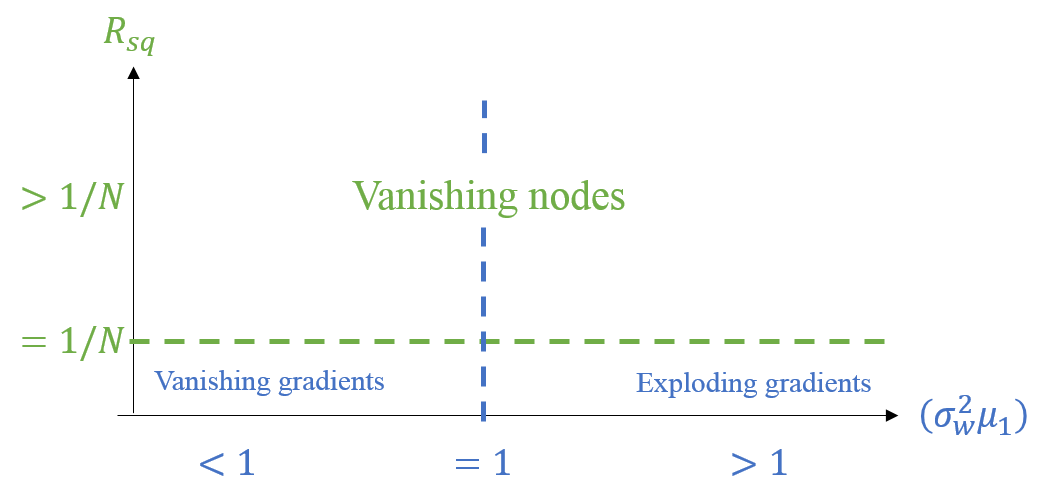
\includegraphics[width=0.7\textwidth]{theo}
\caption{The schematic diagram for deep neural network architectures. To avoid the network from exploding/vanishing gradients and vanishing nodes as the network depth $L$ goes deeper, the best network setting is located at the intersection of vertical and horizontal dashed line.}
\label{fig:sec6_theo1}
\setlength{\belowcaptionskip}{-10pt}
\end{figure}


% According to \eqref{rsq_eigen}, if $R_{sq}$ gets larger, then $m_2$ is also larger compared to $m_1^2$. Recall that $m_i$ is the $i$-th moment of eigenvalues of $\mathbf{JJ}^T$, so the variance of eigenvalues of $\mathbf{JJ}^T$ is $m_2-m_1^2$. Also, eigenvalues of $\mathbf{JJ}^T$ is equivalent to the squared singular values of $\mathbf{J}$. Thus, if the variance of eigenvalues of $\mathbf{JJ}^T$ is too big, the Jacobian $\mathbf{J}$ will become ill-conditioned. Therefore, we can relate $R_{sq}$ to the condition number of Jacobian $\mathbf{J}$, and thus we can link the vanishing node problem to the ill-conditioned Jacobian, which is emphasized in previous works (\cite{mft:sigmoid, mft:spectral, mft:linear}).

% Moreover, \textit{dynamical isometry}, a stronger condition for deep neural networks, is described as "\textit{all} singular values of the Jacobian concentrate near 1" by \cite{mft:sigmoid, mft:linear}. That is, if \textit{dynamical isometry} is achieved, then the variance of singular values of the input-output Jacobian will approach nearly zero, which implies $m_2-m_1^2\approx 0$. Therefore, the $R_{sq}$ will also remain nearly $1/N$ even at a large depth $L$.

% Therefore, we can say that dynamical isometry is not only related to the \textit{learning speed} (\cite{mft:linear}), but also linked to the node correlation $R_{sq}$, which is closely connected with the \textit{learning capability} and the \textit{representation power} of a deep neural network.


%% Below are our numerical results about layer-wise forward and backward variances. As the simulation we have performed in Section 5, we can see that the variances are neither exploding nor vanishing though the nodes in the network are already highly correlated.

% \begin{figure}
    \begin{minipage}[c]{0.67\textwidth}
        \includegraphics[width=\textwidth]{"NodeHistogram"}
    \end{minipage}\hfill
    \begin{minipage}[c]{0.3\textwidth}
        \caption{To show that node vanishing is not arise from gradients exploding or vanishing, we plot histograms of hidden nodes of the updated network in figure \ref{fig:sec5_sim2}. We can observe that the scales of hidden nodes are neither vanishing nor exploding.}
        \label{fig:sec6_sim1}
    \end{minipage}
\end{figure}

